\section{Конструкторская часть}

\subsection{Реализация алгоритма обратной трассировки лучей}

\subsubsection{Алгоритм обратной трассировки лучей}

Алгоритм обратной трассировки лучей работает следующим образом: из камеры пускается луч через каждый пиксель экрана и ищется его пересечения с объектами сцены. Луч выпущенный из камеры называется первичным. Пусть точка пересечения называется П1.

\begin{figure}[hbtp]
	\centering
	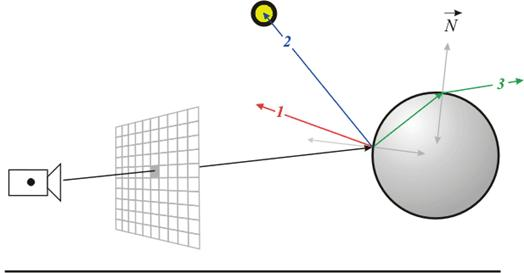
\includegraphics[scale=0.8]{img/trace_2.jpg}
	\caption{Схема работы алгоритма трассировки лучей}
	\label{fig:trace}
\end{figure}				

Далее для каждого источника света определяется, видна ли для него точка П1. Для это испускается теневой луч(луч 2) из П1. Если он пересекается с какими-либо объектами, находящимися между П1 и источником света, то точка находится в тени от это источника и не освещается им. Далее освещение считается по модели. Результатом будет сумма интенсивностей всех видимых источников света для П1. Если материал имеет отражающие свойства то просчитывается и испускается отражённый луч света(луч 1) и точно так же рекурсивно обрабатывается. Аналогично происходит с преломлёнными лучами(луч 3), если материал имеет преломляющие свойства.

\begin{figure}[hbtp]
	\centering
	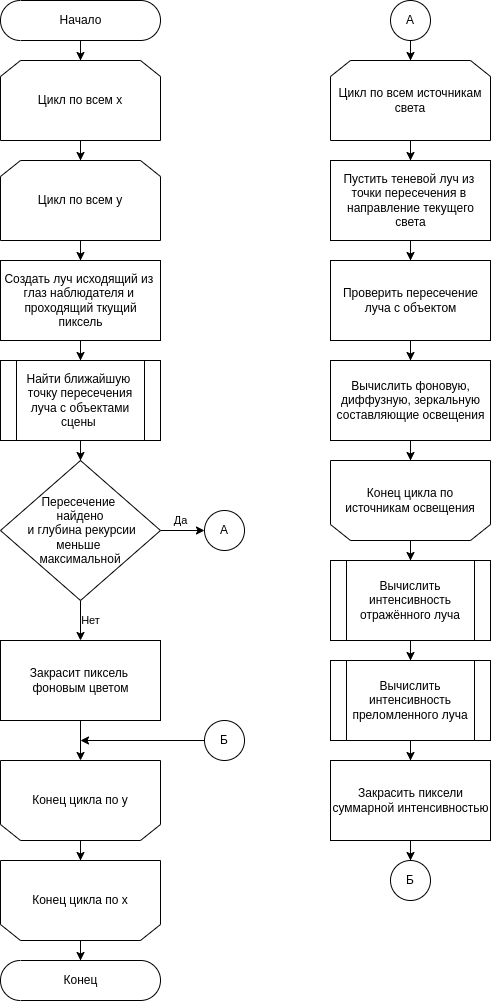
\includegraphics[scale=0.65]{img/trace_diag.png}
	\caption{Блок-схема алгоритма трассировки лучей}
\end{figure}

\newpage	
\subsubsection{Нахождение пересечения с полигоном}

Самым известным тестом на пресечение луча и треугольника является барицентрический тест.

\begin{figure}[h]
	\centering
	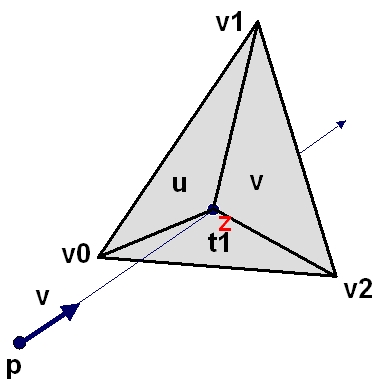
\includegraphics{img/intersec.jpg}
	\caption{Схема для поиска пересечения луча и треугольника}
	\label{fig:intersec}
\end{figure}

Введём следующие обозначения как на рисунке \ref{fig:intersec}

\begin{itemize}
	\item $Z$ - точка пересечения;
	\item $P$ - начало луча;
	\item $t$ - расстояние от $p$ до $z$;
	\item $\vec{d}$ - направление луча;
	\item $V_{0}$, $V_{1}$, $V_{2}$ - вершины треугольника;
	\item $u$, $v$, $t1$ - барицентрические координаты.
\end{itemize}

Барицентрические координаты представляют собой отношения площадей маленьких треугольников к большому треугольнику. Имея 3 точки на плоскости, можно выразить любую другую точку через ее барицентричечкие координаты. Если каждая из этих координат будет больше или равна нулю, то искомая точка принадлежит треугольнику.\cite{intersec}
 
\begin{equation}
	Z(u, v) = (1 - u - v)*V_{1} + u*V_{2} + v*V_{0}
	\label{eq:1}
\end{equation}

Уравнение (\ref{eq:1}) берется просто из определения барицентрических координат, выражая точку пересечения z.

\begin{equation}
	Z(t) = P + t*\vec{d}
	\label{eq:2}
\end{equation}

Уравнение (\ref{eq:2}) это параметрическое уравнение прямой.

\begin{equation}
	P + t*\vec{d} = (1 - u - v)*V_{1} + u*V_{2} + v*V_{0}
	\label{eq:3}
\end{equation}

Приравняв правые части уравнений (\ref{eq:2}) и (\ref{eq:3}) получаем третье уравнение, которое, по сути, является системой из 3-х уравнений с 3-мя неизвестными ($u$ ,$v$, $t$).

Проведя алгебраические преобразования получим
\[
\begin{bmatrix}
	t\\
	u\\
	v
\end{bmatrix}
= \frac{1}{(\vec{V}, \vec{E_{1}})}*
\begin{bmatrix}
	(\vec{Q}, \vec{E_{2}})\\
	(\vec{V}, \vec{T})\\
	(\vec{Q}, \vec{d})
\end{bmatrix}
\]
где $\vec{E_{1}} = V_{1} - V_{0}, \vec{E_{2}} = V_{2} - V_{0}, \vec{T} = P - V_{0}, \vec{V} = (\vec{d} \times \vec{E_{2}}), \vec{Q} = (\vec{T} \times \vec{E_{1}})$.

\subsubsection{Нахождение пересечения с объемлющей оболочкой}

При трассировке лучей крайне неэффективно искать пересечения с каждым полигоном объекта. Лучше поместить объект в объемлющею оболочку и сначала проверять пересечение с ней. Если луч не пересекает оболочку, то и не пересекает объект сцены, находящийся в оболочке. В качестве такой оболочки будет использоваться сфера в связи с простотой поиска пересечения луча и сферы.

\begin{figure}[htp]
	\centering
	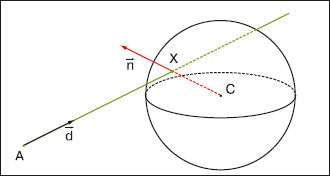
\includegraphics{img/sphere.png}
	\caption{Пересечение сферы лучём}
	\label{fig:sphere}
\end{figure}	

Из уравнение луча имеем $X = A + t\vec{d}$. Уравнение для точки на поверхности сферы выглядит следующим образом $|X - C|^2 = r^2$. Подставив $X$ во второе уравнение получаем: 
\[
|A + t\vec{d} - C|^2 = r^2
\]

Обозначим $\vec{s} = A - C$, тогда

\[
|s + t\vec{d}|^2 = (\vec{s}, \vec{s}) + 2t*(\vec{s}, \vec{d}) + t^2*(\vec{d}, \vec{d}) = r^2
\]

Получилось квадратное уравнение относительно t. Дискриминант считается считается следующим образом:

\[
D = 4*((\vec{s}, \vec{d})^2 - d^2*(s^2 - r^2))    				
\]

%\begin{equation}				
%t_{1,2} = \frac{-(s, d) +- \sqrt{(s, d)^2 - d^2*(s^2 - r^2)}}{d^2}
%5\label{eq:8}
%\end{equation}

Если D < 0 то объект, находящийся в объемлющей сфере, сразу можно выбрсывать из рассмотрения, так как луч его точно не пересекает.

\subsubsection{Ускорение алгоритма трассировки лучей}

Распараллеливание алгоритмов часто используют для ускорения работы. Алгоритм трассировки лучей отлично поддаётся распраллеливанию, поскольку каждый пиксель экрана обрабатывается независимо. Можно разбить экран на сектора в виде прямоугольников, которые будут обрабатываться параллельно, независимо друг от  друга. Также можно строить иерахическую структуру оболочек, что позволит отбрасывать сразу целые группы объектов, которые не пересекает данный луч \cite{trace}.

\subsection{Реализация модели освещения Уиттеда}

\subsubsection{Нахождение отражённого луча}

Для нахождения направление отражённого луча $\vec{R}$ необходимо знать только направления нормали $\vec{N}$ и падающего луча $\vec{L}$.

\begin{figure}[htp]
	\centering
	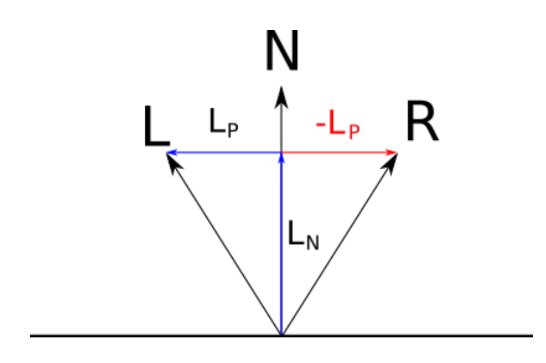
\includegraphics[scale=0.5]{img/reflect.png}
	\caption{Разложение падающего луча}
	\label{fig:reflect}
\end{figure}

Падающий вектор $\vec{L}$ можно разложить на два проекции $\vec{L_{N}}$ и $\vec{L_{P}}$. Тогда $\vec{L} = \vec{L_{N}} + \vec{L_{P}}$. Так как $\vec{N}$ единичный вектор, то длинна прекции будет равна $(\vec{L}, \vec{N})$ и $\vec{L_{N}} = (\vec{L}, \vec{N})\vec{N}$. Следовательно $\vec{L_{P}} = \vec{L} - \vec{L_{N}}$. Отражённый же луч можно выразить как $\vec{R} = \vec{L_{N}} - \vec{L_{P}}$. Всё подставивив и упростив окончательно получаем $\vec{R} = 2(\vec{L}, \vec{N})\vec{N} - \vec{L}$.

\subsubsection{Нахождение преломлённого луча}

Преломлённый луч $\vec{P}$ можно найти изходя их того факта что падающий и преломлённый лучи лежат в одной плоскости и из закона Снелиуса, который записывается так:

\[
sin(\alpha)*n_{1} = sin(\gamma)*n_{2}
\label{eq:9}
\] 

\begin{figure}[htp]
	\centering
	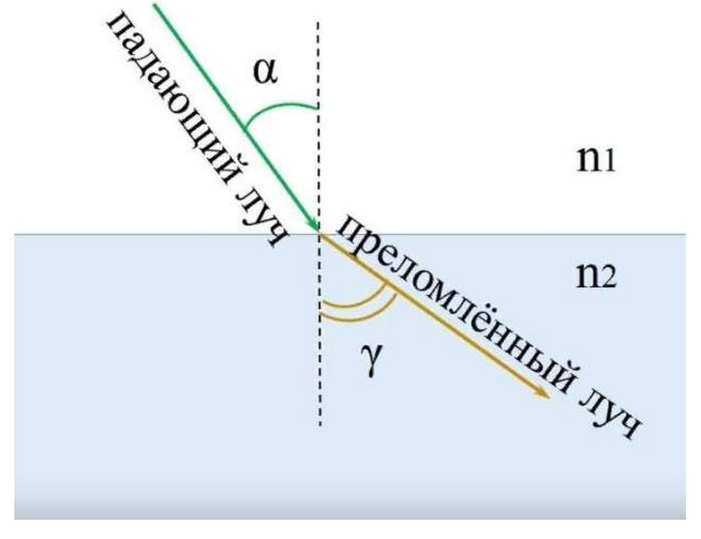
\includegraphics[scale=0.35]{img/refract.png}
	\caption{Преломление}
	\label{fig:refract}
\end{figure}

Введём дополнительные обозначение $n = \frac{n_{1}}{n_{2}}$, $\vec{L}$ - падающий луч, $\vec{N}$ - нормаль. Можем получить уравнение для вектора преломлённого луча:

\[
\vec{P} = n*(\vec{L} + cos(\alpha)*\vec{N}) - \vec{N}\sqrt{1 - sin^2(\gamma)}
\]

Если подкоренное выражение отрицательно, то этот случай соответствует полному отражению.	

\subsubsection{Общая реализация модели освещения Уиттеда}

Модель Уиттеда учитывает фоновое, диффузное и зеркальное освещение, а также эффекты отражения и преломления, рекурсивно вычисляя интенсивность этих лучей. Согласно этой модели суммарная интенсивность определяется уравнением \ref{eq:whitted_general}.

\subsubsection{Расчёт интенсивностей}

Интенсивность диффузного отражения не зависит от положения наблюдателя. Её интенсивность в точке можно вычислить по следующей формуле:
\[
I_{d} = k_{d} * \sum I_{i}*(\vec{N}, \vec{L_{i}}),
\]
где 
\begin{itemize}
	\item[---] $k_{d}$ - коэффициент диффузного отражения;
	\item[---] $I_{i}$ - интенсивность в точке, от i-го источника света;
	\item[---] $\vec{N}$ - нормаль;
	\item[---] $\vec{L_{i}}$ - единичный вектор, направленный в строну i-го источника света.
\end{itemize}

Интенсивность же зеркального отражения зависит от положения наблюдателья и её интенсивность в точке можно вычислить по следующей формуле:
\[
I_{d} = k_{s} * \sum I_{i}*(\vec{S}, \vec{R_{i}})^n,
\]
где 
\begin{itemize}
	\item[---] $k_{s}$ - коэффициент зеркального отражения;
	\item[---] $I_{i}$ - интенсивность в точке, от i-го источника света;
	\item[---] $\vec{S}$ - единичный вектор, направленный в строну наблюдателя;
	\item[---] $\vec{R_{i}}$ - единичный вектор, задающий направленние отражённого луча от i-го источника света;
	\item[---] $n$ - степень, аппроксимирующая пространственное распределение зеркально отраженного света.
\end{itemize}

В итоге получается следующая формула:
\[
I = k_{a} \sum I_{ai} + k_{d} * \sum I_{i}*(\vec{N}, \vec{L_{i}}) + k_{s} * \sum I_{i}*(\vec{S}, \vec{R_{i}})^n + k_{r}I_{r} + k_{t}I_{t},
\]

\subsection{Выбор используемых типов данных}

В программе будут реализованны и использованны следующие структуры данных:
\begin{itemize}
	\item[---] Point3D - точка;
	\item[---] Vector3D - вектор;
	\item[---] Color - цвет;
	\item[---] Polygon - полигон. Хранит индексы вершин, нормалей и  текстурных координат;
	\item[---] SceneObject - объект сцены. Хранит вершины, нормали, текстурные координаты и полигоны;
	\item[---] LightObject - источник света. Хранит координаты источника света;
	\item[---] Camera - камера. Хранит координаты, направление и вектор указывающий наверх;
	\item[---] Scene - сцена. Хранит все объекты.
\end{itemize}

\pagebreak